% !TEX root = ../thesis.tex
\chapter{基于自适应相似性的深度抠图方法}
\section{引言}
在前几章中,我们分别研究了数据驱动的相似性学习在无监督的度量学习和半监督的约束聚类中的应用情况,本章将着重研究相似性学习在具有监督信息的自然图像抠图问题中的算法应用。

自然图像抠图(natural image matting)是计算机视觉中的重要任务之一。它在图像或视频编辑、合成和电影后期制作方面具有大量应用\cite{wang2008image,aksoy2017designing,lutz2018alphagan,xu2017deep,samplenet}。抠图问题已引起学术界的极大兴趣,并且在过去十年中被广泛地研究。
自然图像抠图是将前景对象与背景图相分离的问题并估计它们之间的过渡取值的问题。数字图像抠图将输入的自然图像视为前景图和背景图的合成图像,旨在估计前景图像的不透明度。其预测结果是alpha半透明遮罩(alpha matte),表示每个像素在前景和背景之间的过渡取值\cite{wang2008image}。

在数学形式上,观察到的RGB图像$ I $被建模为前景图像$ F $和背景图像$ B $的凸组合的形式\cite{chuang2001bayesian,wang2008image}:
\begin{equation}
I_p = \alpha_pF_p + (1-\alpha_p)B_p, \quad \alpha_p \in [0,1],
\label{eq5:matting}
\end{equation}
其中$ \alpha_p $表示要在像素位置$ p $所估计的alpha遮罩值。如果$ \alpha_p $的取值不是$0$或者$1$,则在像素位置$p$的图像像素值即是由前景和背景混合而成。由于前景颜色$ F_p $、背景颜色$ B_p $和alpha取值$ \alpha_p $都是未知的,所以图像抠图的原始数学定义是一个欠定问题。因此,大多数先前的传统抠图算法都会在抠图问题中引入一个比较强的归纳偏置(inductive bias)。同时,在大多数抠图任务中,都将trimap图像作为粗略标注提供给算法,trimap图像上标注有已知的前景和背景区域以及需要预测的未知区域。

在基于相似性和基于采样的算法中广泛采用的基本思想之一是从具有相似外观的图像区域中借用信息。通常,传统的基于相似性的方法\cite{levin2008closed,he2010fast,chen2013knn,aksoy2017designing}通过参考输入图像中不同区块间的外观相似性,将不透明度或透明度在像素之间进行传播,以生成alpha遮罩值。基于采样的算法\cite{wang2007optimized,gastal2010shared,he2011global,feng2016cluster}一般从前景和背景中借用一对采样区块,以基于某些特定假设来估计未知区域中每个像素的alpha值。
先前基于相似性和基于采样的方法的一个不足点是,它们无法处理trimap中仅存在背景区域和未知区域标注的情况。这是因为这些方法必须同时利用前景和背景信息来估计alpha取值,在没有前景标注的情况下,这些算法无法正常计算。

受益于Adobe Image Matting数据集\cite{xu2017deep},近年来出现了更多基于学习的图像抠图方法 \cite{xu2017deep,lutz2018alphagan,lu2019indices,samplenet,cai2019disentangled,hou2019context}。大多数基于学习的方法都使用神经网络先验作为归纳偏置并直接预测Alpha遮罩值。

部分基于深度学习的抠图方法\cite{samplenet,cai2019disentangled}更是潜在地利用了相似外观的图像区域具有相似alpha遮罩值这一假设作为归纳偏置,从而改进了其抠图效果。
SampleNet\cite{samplenet}通过其方法中采用的图像补全(image inpainting)网络\cite{yu2018generative}实现传播,以进行前景和背景估计,再通过采样方法预测alpha值,而不是通过传播不透明度直接进行预测。此外,图像补全网络中的传播行为仅作用在具有强语义的少部分特征上,而不是在高分辨率特征上进行。在AdaMatting\cite{cai2019disentangled}中,作者将卷积长短时记忆(Convolutional LSTM,ConvLSTM)网络\cite{xingjian2015convolutional}引入了它们的网络中,作为网络最后的传播阶段。其中,信息传播是基于ConvLSTM中的卷积和记忆存储部分实现的。
ConvLSTM和直接传播之间并不能看作是等价的计算模块,两者的区别可以类比于LSTM\cite{hochreiter1997long}和transformer\cite{vaswani2017attention}之间的区别。

在本章中,我们将先后提出两种基于相似性的深度抠图方法。首先将提出基本的引导上下文注意力抠图(Guided Contextual Attention Matting,GCA Matting)模型,以在深度神经网络中实现基本的信息传播功能。然后在此基础上提出了一种新颖的层次化不透明度传播(Hierarchical Opacity Propagation,HOP)方法,其中,不透明消息可以在不同语义级别的特征间进行传播。近几年信息传播在神经网络框架中被广泛地采纳,从自然语言处理\cite{vaswani2017attention,yang2019xlnet},数据挖掘\cite{kipf2016semi,velivckovic2017graph}到计算机视觉\cite{yu2018generative,wang2018non}都有大量工作通过信息传播的方式改进算法性能。所提出的结构主要由全局HOP模块和局部HOP模块两种传播模块构成。HOP模块基于所提出的引导上下文注意力(Guided Contextual Attention,GCA)机制实现,该机制可以在全卷积神经网络中模拟基于相似性的传统抠图算法的传播过程。在GCA机制中,低级语义特征被用来作为传播过程的引导信息,根据引导信息,该机制对alpha特征进行传播。已知区块和未知区块中的信息被传播到未知区域中具有相似外观的特征区块中。

本章中所提出的图像抠图方法可以从两个不同的角度进行解释。 一方面,可以将引导上下文注意力机制解释为一种具有神经网络先验的基于相似性进行alpha值传播的抠图方法。在低级图像特征间相似度的引导下,未知区域中的区块相互之间对具有高级语义的alpha特征进行共享。
另一方面,所提出的方法也可以看作是引导性的图像补全任务。在这个角度下,根据输入图像的引导,图像抠图任务可以被视为是在alpha遮罩图像上的补全任务。未知区域类比于要在图像补全中待填充的孔洞部分。与通常情况下,从同一图像的背景借用像素的补全方法不同的是,图像抠图在原始RGB图像的引导下在alpha遮罩图像中的已知区域借像素值$ 0 $或$ 1 $来填充未知区域。

\section{相关工作}
大多数自然图像抠图方法可以粗略分为基于相似性的方法\cite{levin2008closed,he2010fast,lee2011nonlocal,chen2013knn,aksoy2017designing},基于采样的方法\cite{wang2007optimized,gastal2010shared,he2011global,feng2016cluster}和基于学习的方法\cite{xu2017deep,lutz2018alphagan,lu2019indices,samplenet,hou2019context,cai2019disentangled}三类。在本节中,我们将回顾一些与该章节相关度较高的基于深度学习的抠图算法。

一般基于深度学习的方法利用深度神经网络通过给定图像和trimap图直接预测alpha遮罩值。
Cho等人\cite{cho2019deep}最先在抠图任务中使用了端到端卷积神经网络(Convolutional Neural Network,CNN),该网络从Closed-form Matting\cite{levin2008closed}和KNN Matting\cite{chen2013knn}中获取alpha值以及归一化的RGB图像作为输入,以更好地利用局部和非局部(nonlocal)结构信息对不同算法生成的alpha值进行融合。
文献\parencite{xu2017deep}中提出了Deep Matting方法作为一个两阶段网络来预测alpha遮罩。在第一阶段中,算法向深层卷积编码器-解码器网络输入图像和相应的trimap,得到粗略预测结果。在第二阶段,通过浅层网络对粗略预测的alpha值进行细化。
Lutz等人\cite{lutz2018alphagan}将生成对抗网络(Generative Adversarial Networks,GAN)引入了图像抠图问题,并使用膨胀卷积来捕获全局上下文信息。
Tang等人\cite{tang2019very}提出了一个名为VDRN的神经网络,该网络包含一个深度残差(residual)编码器和一个复杂的解码器。
AdaMatting\cite{cai2019disentangled}方法将抠图问题分为两个任务,trimap自适应和alpha估计,并使用具有两个不同解码器分支的CNN模型以多任务学习方式处理。
IndexNet Matting\cite{lu2019indices}方法将池化(pooling)操作中的索引作为特征图的函数,并提出了一种通过索引引导的编码器-解码器网络,该网络通过由学习得到的索引信息进行的索引池化和上采样。
Hou和Liu\cite{hou2019context}提出了一个上下文感知(context-aware)网络来预测前景和alpha遮罩值。Context-aware Matting使用两种编码器,一种用于局部特征,另一种用于上下文信息。 

一些方法表明,不对alpha进行直接预测,而更改问题的自由度可以改善网络的性能。
Tang等人\cite{samplenet}提出了SampleNet来逐步地估计前景、背景和alpha遮罩,而不是同时对其进行预测。
Zhang等人\cite{Zhang2019ALF}使用两个解码器分支分别估计前景和背景,然后使用融合分支获得最终预测结果。

上面提到的绝大多数方法都严重依赖trimap作为输入,以减小解空间。然而最近,对于特定的实际问题,一些利用图像语义信息可以在没有任何trimap图输入的情况下具有良好抠图效果的方法被陆续提出。
Shen等人\cite{shen2016deep}将端到端CNN与Closed-form Matting\cite{levin2008closed}结合起来,自动生成人像的trimap图,然后获得所需的alpha遮罩值。
Chen等人\cite{chen2018semantic}提出了一种语义人体抠图(Semantic Human Matting,SHM)方法,将语义分割网络与抠图网络集成在一起以自动提取人体的alpha遮罩。

\section{深度图像抠图基线网络}
我们所提出的模型使用带有GCA机制的HOP模块以及一个自定义的U-Net\cite{ronneberger2015u}架构实现深度自然图像抠图。在本节中,我们将首先对自定义的U-Net基线网络进行介绍。

\begin{figure}[t]
	\centering
	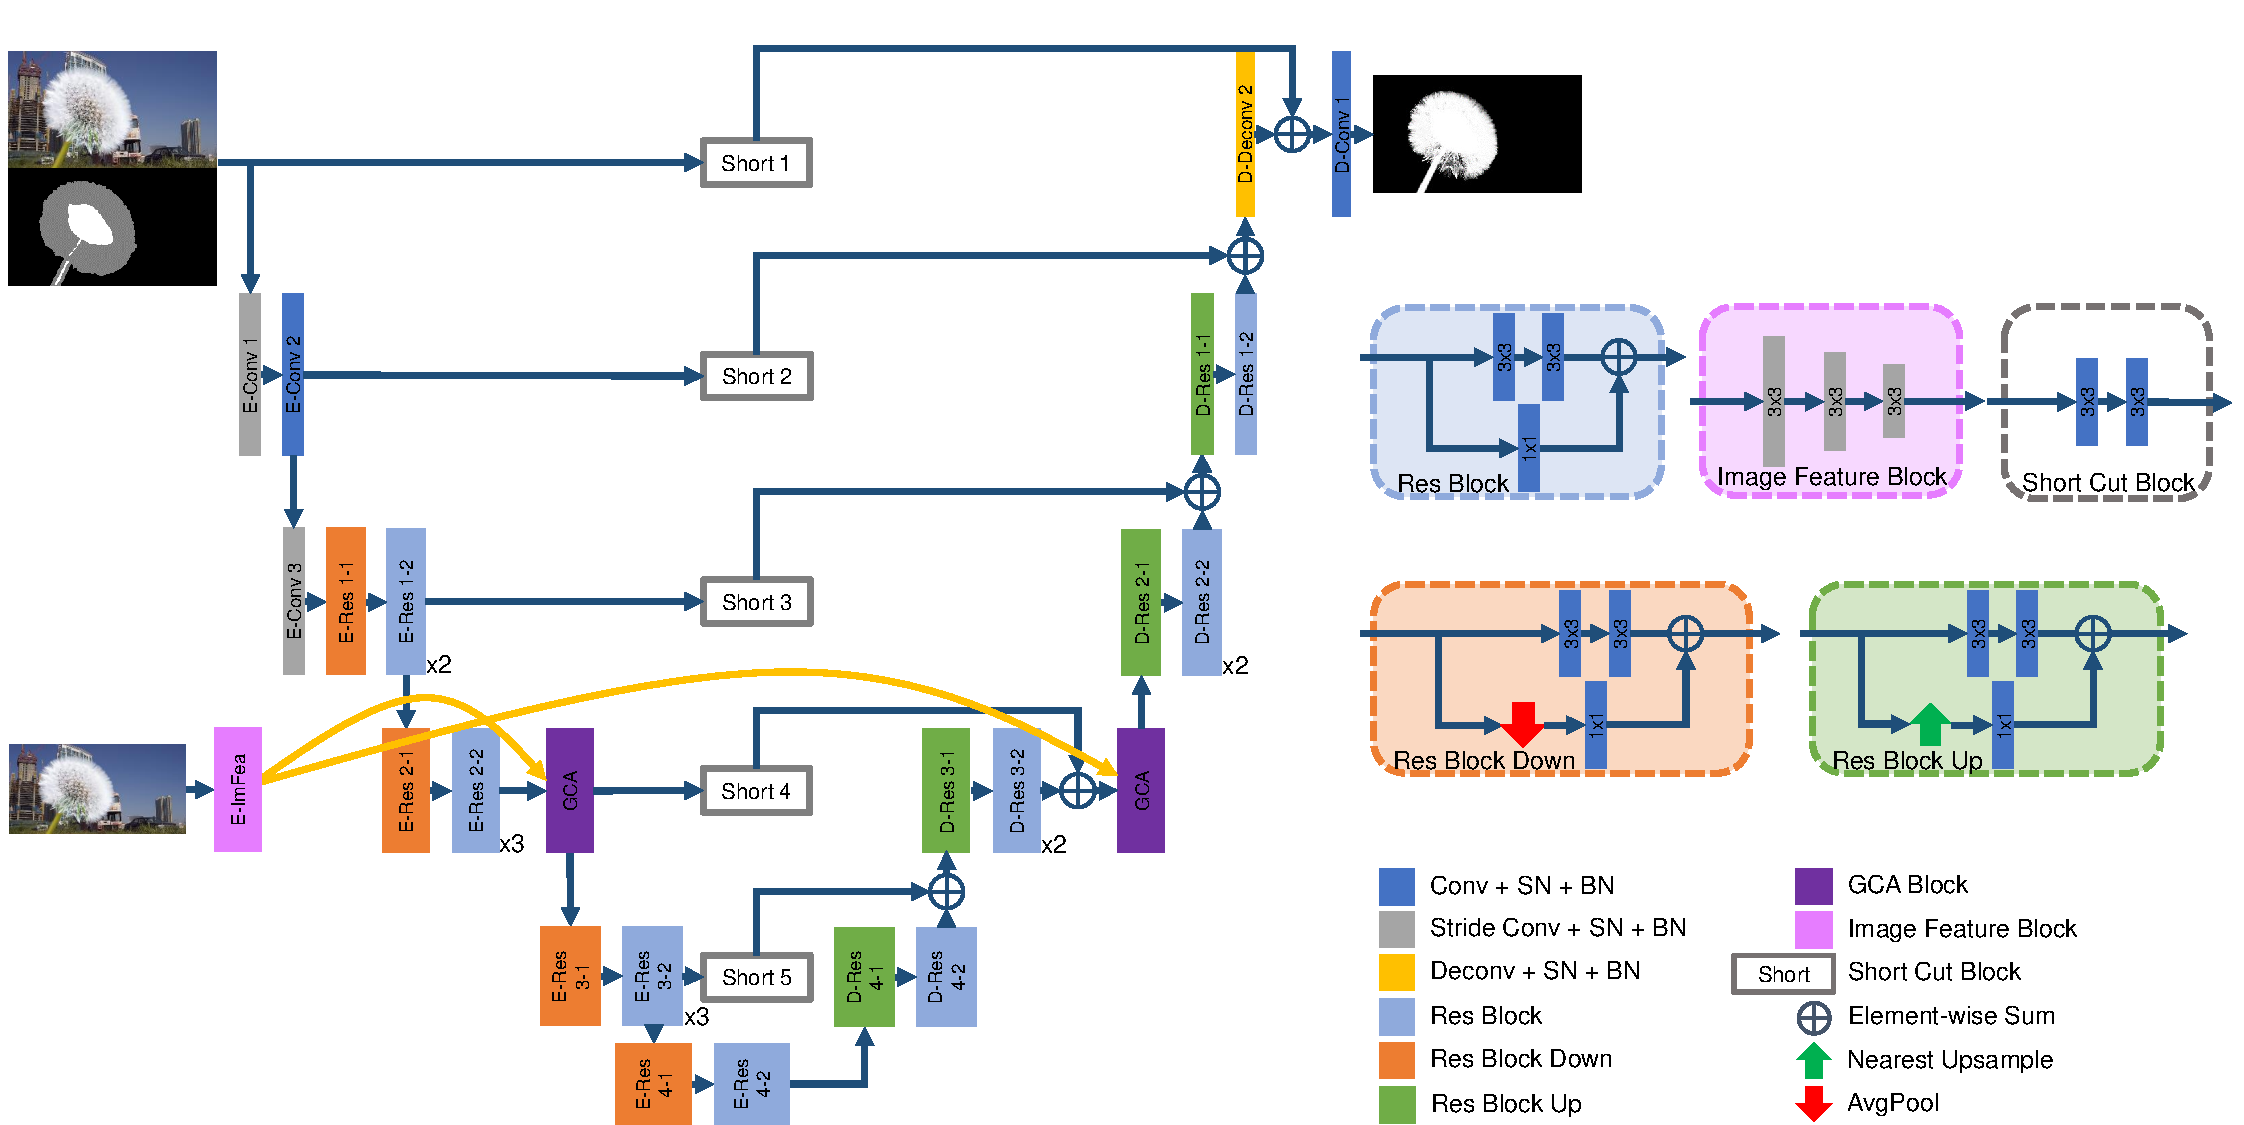
\includegraphics[width = 1\textwidth]{chap5/10261arch1.pdf}
	\bicaption{所提出的GCA Matting的网络结构细节图。基线网络模型具有相同的网络结构,但不具备图中的GCA机制部分以及图像特征模块。原始图像和trimap图像为alpha特征的输入数据,而图像特征模块仅将原始的合成图像作为输入数据。蓝色箭头表示alpha特征流,黄色箭头表示低级语义的图像特征流。GCA:引导上下文注意力;SN:谱归一化;BN:批归一化; $ \times N $:重复$ N $次}{Overview of our proposed guided contextual attention matting framework. The baseline model shares the same architecture without GCA mechanism and image feature block. Original image and trimap are the inputs of alpha feature. Image feature block only takes the original merged image as input. The blue arrows denote alpha feature flow and yellow arrows denote low-level image feature flow. GCA: guided contextual attention; SN: spectral normalization; BN: batch normalization; $ \times N $: replicate $ N $ times}
	\label{fig5:arch}
\end{figure}

\subsection{基线网络结构}
在近几年的图像抠图\cite{lutz2018alphagan,samplenet,lu2019indices}、图像分割\cite{long2015fully}、图像转换\cite{isola2017image}和图像补全\cite{liu2018image}任务中,类U-Net网络结构非常流行。在图\ref{fig5:arch}中给出了具有附带的GCA机制的基线网络结构。图中的网络结构与我们所设计的基线网络模型的唯一区别在于基线网络中没有GCA机制,因此也就没有其上游的图像特征模块(Image Feature Block)。

该基线网络的输入为裁剪后的图像块和3通道独热编码(one-hot encoding)的trimap图,它们被拼接为一个6通道输入。输出是相应的预测alpha遮罩值。
基线网络结构被设计为具有堆叠残差模块(stacked residual blocks)\cite{he2016deep}的编码器-解码器网络。

由于低级图像特征能对在alpha遮罩中保留纹理信息起到至关重要的作用,因此在我们自定义的基线模型中,解码器在上采样块之前(而不是在每个上采样块之后)对编码器输出的特征进行合并。这是因为预期中这些编码器特征具有更多的低级图像特征,而这样的设计可以避免在低级特征上进行更多的卷积计算。我们还使用了具有两层卷积层的跳层(short cut)块来对齐编码器特征的通道以进行特征融合。同时,与仅结合了不同的中级特征的典型U-Net结构不同,我们将原始输入直接通过跳层块传递到最后的卷积层。这些特征不与主干网络共享任何计算。因此,此跳层分支仅关注细节上的的纹理和梯度信息。

除了广泛使用的批归一化\cite{ioffe2015batch},我们还将谱归一化\cite{miyato2018spectral}引入每个卷积层,以对网络的Lipschitz常数添加约束达到稳定训练的效果,该设计方案普遍存在于图像生成任务中\cite{brock2018large,zhang2018self}。

\subsection{损失函数}
在所提出的神经网络的训练中,我们仅使用了一个alpha预测损失。alpha预测损失可以定义为每个像素的alpha预测值和标注的真实值之间的绝对差在整个未知区域上的平均值:
\begin{equation}
\mathcal{L} = \frac{1}{|\mathcal{U}|} \sum_{i\in \mathcal{U}}|\hat{\alpha_i}-\alpha_i|,
\end{equation}
其中$ \mathcal {U} $表示在trimap中标记为未知区域的像素集合,$ \hat{\alpha_i} $和$ \alpha_i $分别表示像素位置$ i $的alpha遮罩预测值和真实值。

在先前的部分相关工作中,针对深度图像抠图任务,有一些新的损失函数被提出来,例如合成损失函数\cite{xu2017deep},梯度损失函数\cite{samplenet}和Gabor损失函数\cite{li2019inductive}。
Deep Matting\cite{xu2017deep}中使用的合成损失函数是通过计算由真实前景,背景和预测alpha遮罩所合成的预测图像与原始输入图像之间的绝对差作为损失。
梯度损失计算未知区域中alpha预测值梯度和真实值梯度之间的平均绝对差。
文献\parencite{li2019inductive}中提出的Gabor损失通过用一系列Gabor过滤器代替了梯度损失中的梯度算子,旨在能在纹理和梯度方面提供比梯度损失更全面的监督。

我们对这些损失进行了深入的研究,以揭示添加这些不同的损失是否可以使基线模型中的alpha值预测效果得到提升。我们在表\ref{tab5:ablation}中提供了在Composition-1k测试集\cite{xu2017deep}上进行的消融实验结果。如表\ref{tab5:ablation}所示,对预测结果的MSE和Gradient评测误差而言,引入合成损失函数不会带来任何显着差异,并且当我们将梯度损失加入到alpha预测损失时,给出的两种评测误差都会增加。尽管采用Gabor损失可以在一定程度上Gradient梯度误差,但也会稍微提高MSE结果。因此,我们仅在模型中选择alpha预测损失作为唯一的损失函数。


\begin{table}[t]
	\bicaption{基线网络结构上的数据增广和不同损失函数的消融实验结果。定量实验结果测试于Composition-1k测试集。Aug:数据增广;Rec:alpha预测损失;Comp:合成损失;GradL:梯度损失;Gabor:Gabor损失}{Ablation study on data augmentation and different loss functions with baseline structure. The quantitative results are tested on Composition-1k testing set. Aug: data augmentation; Rec: alpha prediction loss; Comp: compositional loss; GradL: gradient loss; Gabor: Gabor loss.}
	\centering
	\setlength{\tabcolsep}{8pt}
	\begin{tabular}{ccccc|cc}  
		\toprule
		Aug&Rec&Comp&GradL&Gabor& MSE & Grad\\% & SAD &Conn
		\midrule
		\checkmark&\checkmark&&& & 0.0106 & 21.53 \\  % & {40.62}& 38.43
		\checkmark&\checkmark&\checkmark&&& 0.0107  & 21.85\\% & 40.85  & 38.73
		\checkmark&\checkmark&&\checkmark& & 0.0108 & 22.51\\ % & 43.62  & 42.19
		\checkmark&\checkmark&&&\checkmark & 0.0109 & 20.66\\ % & 42.53  & 40.84   
		&\checkmark&&& & 0.0146 & 32.01 \\%& 51.15& 51.52
		\bottomrule
	\end{tabular}
	\label{tab5:ablation}
\end{table}

\subsection{数据增广方法}

由于文献\parencite{xu2017deep}中所提出的目前最主要的图像抠图数据集仅包含431个用于训练的前景对象,所以我们将数据增广视为基线模型的必须部分。
本节中我们将对一系列模型训练中使用的数据增广方案进行介绍。

首先,延续\cite{samplenet}中的数据增广方案,我们以0.5的概率在前景图集合中随机选择两个前景物体图像,并将它们叠加组合以获得一个新的前景对象以及一个新的alpha图像作为采样数据。随后,以0.25的概率前景对象和alpha图像的大小将被调整为$640 \times 640 $,这样网络模型几乎可以看到整个前景图像,而不是裁剪后的局部图像块。然后,在前景图像和相应的alpha图像上进行随机的仿射变换。在此仿射变换中,我们定义了随机旋转,缩放,斜切以及垂直和水平翻转。再后,通过5到29中采样随机数作为像素数对alpha图像进行膨胀和腐蚀来生成trimap。获得trimap后,我们分别随机从每个前景图像中、alpha图和trimap图中的对应位置裁剪一个$ 512 \times 512 $的区块,所有裁剪的区块的中心像素都落在trimap图的未知区域上。然后将前景图像转换到HSV空间,并对色度,饱和度和明度分别施加不同的噪声。
最后,我们从MS COCO数据集\cite{lin2014microsoft}中为每个增广后的前景块随机选择一个背景图像,并将其合成为一张图像作为原始输入图像。

为了证明数据增广的有效性,我们进行了一个只包含最少数据增广的实验。在这种情况下,仅保留两个必要的操作,即图像裁剪和trimap图的膨胀生成。此实验中不包括更多的例如随机图像缩放和翻转这些在大多数先前的深度图像抠图方法\cite{xu2017deep,lutz2018alphagan,samplenet,lu2019indices}中被广泛使用的增广方式。我们将此实验设置视为无数据增广。实验结果被列在表\ref{tab5:ablation}中。我们可以看到,在不进行额外数据增广的情况下,我们的基线模型已经可以与Deep Matting方法的效果相媲美。

\section{引导上下文注意力抠图模型}
本节将对所提出的仅包含单层次引导上下文注意力机制的GCA Matting模型进行介绍。完整的引导上下文注意力机制包含两种组件,一个是用于低级图像特征抽取的图像特征提取器,另一个是用于信息传播的引导上下文注意力模块。

\begin{figure}[t]
	\centering
	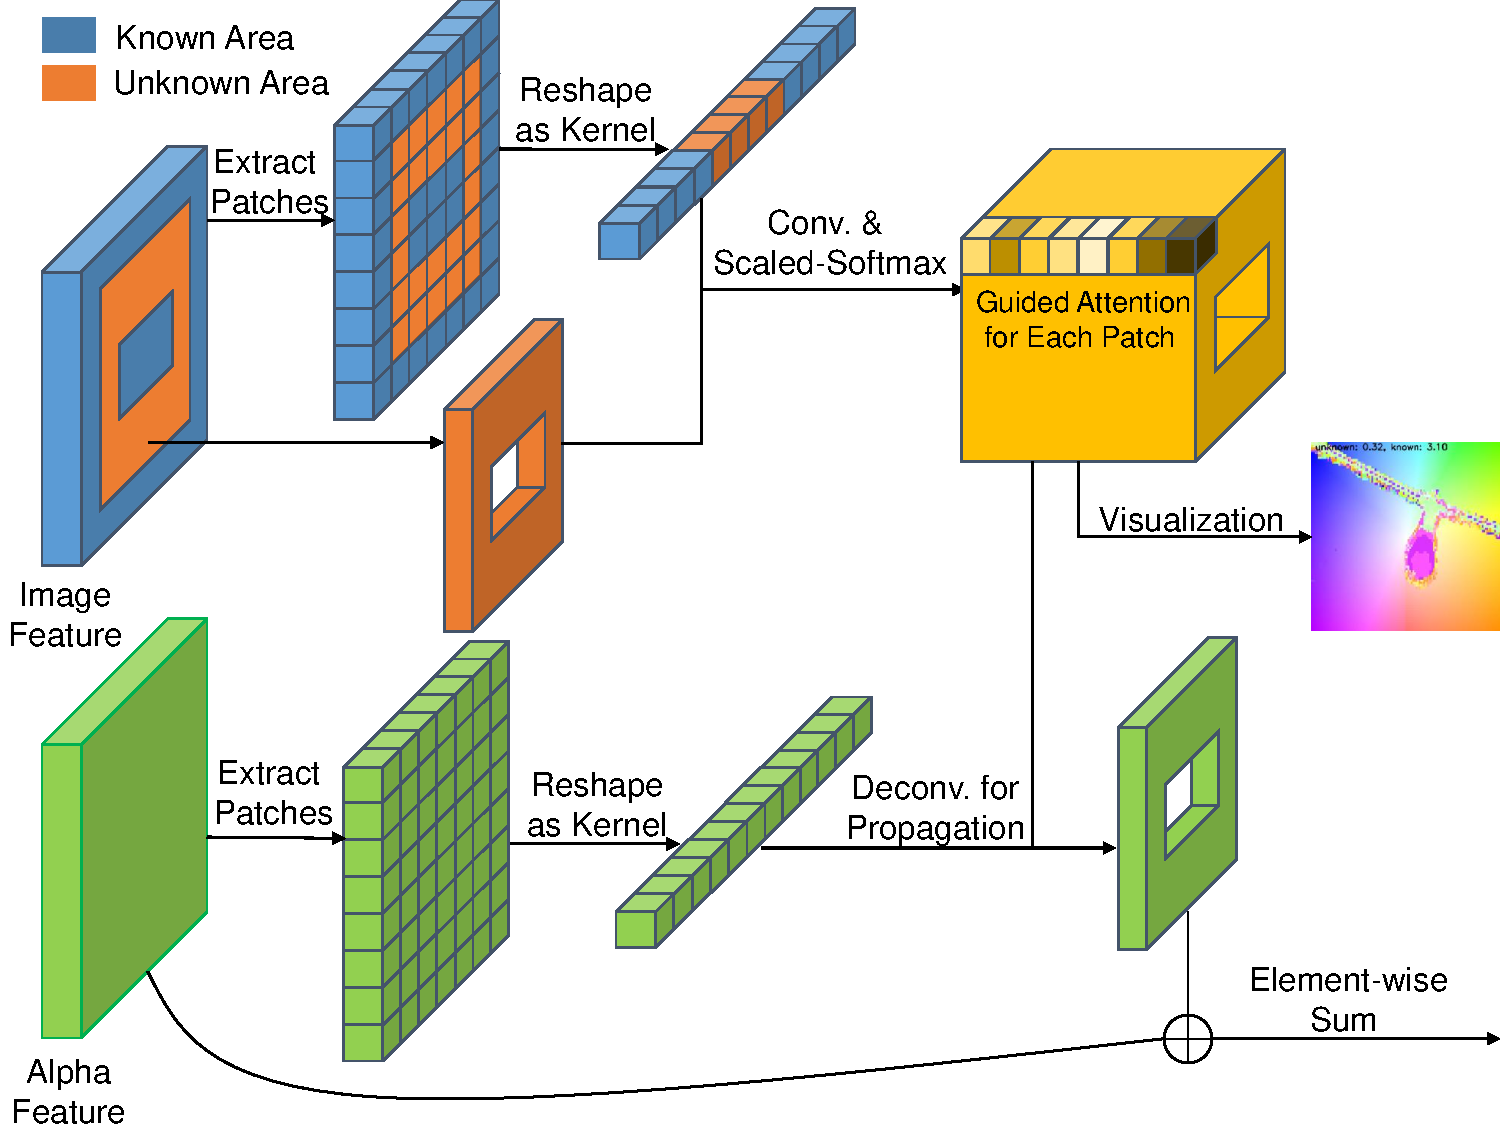
\includegraphics[width = 0.85\columnwidth]{chap5/10261block.pdf}
	\bicaption{引导上下文注意力模块图示。计算过程通过卷积或转置卷积进行实现。为了保持图示整洁,该图中未显示另外两个用于特征对齐的$1\times 1$的卷积层。一个在提取区块之前应用于输入的图像特征,另一个在逐元素求和之前应用于传播结果}{The illustration of the guided contextual attention block. Computation is implemented as a convolution or a deconvolution. Two additional $ 1\times 1 $ convolutional layers for adaptation are not shown in this figure to keep neat. One is applied to the input image feature before extracting patches, and the other one is applied to the result of propagation before the element-wise summation}
	\label{fig5:gca}
\end{figure}

\section{低级图像特征}

大多数基于相似性的方法都具有一个基本的归纳偏置,即外观几乎相同的局部区块应具有相似的不透明度。该归纳偏置允许基于相似性的抠图算法将alpha值从trimap图中的已知区域传播到未知区域,这通常可以产生非常出色的alpha预测效果。

因此,我们在所提出的框架中定义了两个不同的特征流(图\ref{fig5:arch}):alpha特征流(蓝色箭头)和图像特征流(黄色箭头)。其中alpha特征是从由原始图像和trimap图拼接产生的6通道输入生成的。最终的alpha遮罩值可以直接从该特征中预测,故称为alpha特征。低级图像特性与高级alpha特征形成对比,这些特征仅由具有步长(stride)为2的三个卷积层序列从输入图像生成,这类似于传统的基于相似性的方法中所用到的的局部颜色统计量。

具体来说,alpha特征包含不透明度信息,而低级图像特征包含外观信息。
在提供不透明度和外观信息的情况下,GCA机制可以学习到一个前几章中所多次用到的相似性图,并通过类似于基于相似性的抠图方法进行不透明度传播。
换句话说,我们利用低级图像特征来指导alpha特征上的信息流动。

\subsection{引导上下文注意力模块}
受文献\cite{yu2018generative}中上下文注意力模块的激发,我们在抠图问题中引入了引导上下文注意力模块。

如图\ref{fig5:gca}所示,引导上下文注意力同时利用了图像特征和alpha特征。首先图像特征被分为已知部分和未知部分,并从全部的图像特征中抽取$3\times 3$的区块。每个特征块表示一个特定未知的外观信息。我们将特征块变形为卷积核。为了能够对一个中心$ (x,y)$在未知区域的图像特征块$ U_{x,y} $和一个中心在$ (x',y') $的图像特征块$ I_{x', y'} $之间的相关性进行度量,相似性被定义为归一化的内积形式:
\begin{equation}
	s_{(x,y), (x',y')} = 	
	\begin{cases}
	\lambda \quad &(x,y)=(x',y');\\
	\langle \frac{U_{x, y}}{\|U_{x, y}\|},\frac{I_{x', y'}}{\|I_{x', y'}\|}\rangle \quad &\mathrm{otherwise},	
	\end{cases}
\end{equation}
其中$ U_{x, y}\in\mathcal{U}$也是图像特征块集合 $ \mathcal{I} $中的一个元素,即$ \mathcal{U} \subseteq \mathcal{I} $。常数$ \lambda $ 为惩罚参数,可以避免未知区域的特征块和自身之间产生很大的相关性,在模型中我们采用$ \lambda =-10^4$。在实现中,该相关性可以通过未知区域特征块与图像特征块经由变形生成的卷积核进行卷积计算得到。给定一个相关性,则可以在$ (x',y') $维度上进行归一化指数函数(softmax)计算,得到每个特征区块上的引导注意力值:
\begin{equation}
	a_{(x,y), (x',y')} = \mathrm{softmax}(w(\mathcal{U}, \mathcal{K}, x',y')s_{(x,y), (x',y')}),
\end{equation}
\begin{equation}
w(\mathcal{U}, \mathcal{K}, x',y') = \begin{cases}
\mathrm{clamp}(\sqrt{\frac{|\mathcal{U}|}{|\mathcal{K}|}}) \quad I_{x',y'} \in \mathcal{U};\\
\mathrm{clamp}(\sqrt{\frac{|\mathcal{K}|}{|\mathcal{U}|}}) \quad I_{x',y'} \in \mathcal{K},
\end{cases}
\label{eq5:weight}
\end{equation}
\begin{equation}
\mathrm{clamp}(\phi) = \mathrm{min}(\mathrm{max}(\phi, 0.1), 10),
\end{equation}
其中$ w(\cdot)$是权重函数,$ \mathcal{K} = \mathcal{I}-\mathcal{U} $是来自已知区域的图像特征块集合。与图像补全任务不同的是,trimap图中未知区域的面积不受任何控制。在许多输入的trimap图中,存在极大的未知区域而几乎没有已知的像素。因此,仅将不透明度信息从已知区域传播到未知部分通常是不可行的。在所提出的引导上下文注意力机制中,我们让未知部分同时借用已知区域和未知区域中的特征。根据每个区域的面积,通过公式(\ref{eq5:weight})中所定义的权重函数,将不同的权重分配给已知和未知的区域。如果已知区域的面积较大,则已知区域的特征块可以传达更准确的外观信息,从而暴露出前景和背景之间的差异,因此,我们将给已知区域特征块分配较大的权重。而如果未知区域的面积很大,则已知区域的图像特征块只会提供一些局部的外观信息,这可能会损害到不透明度的传播,所以,我们将较小的权重分配给已知区域特征块。

当从图像特征得到引导注意力值后,可以根据由引导注意力值所定义的相似性矩阵,在alpha特征上进行信息传播。
与图像特征类似,从alpha特征中提取特征块并将其变形为卷积核。信息传播过程可以通过引导注意力值与变形后的alpha特征块之间的转置卷积计算完成。该转置卷积可在未知区域中重建alpha特征,并对转置卷积中相互覆盖的像素值取平均。最后,我们通过逐元素求和对输入的alpha特征和传播结果进行融合。这种逐元素求和作为一个残差连接可以对模型训练起到稳定作用。

\subsection{带有引导上下文注意力机制的网络细节}
多数基于相似性的经典抠图方法最终产生一个依赖于图拉普拉斯的闭式解\cite{levin2008closed,lee2011nonlocal,chen2013knn}。闭式解可以被看作是信息传播算子的不动点,或者是传播迭代趋于无穷时收敛到的极限值\cite{zhou2004learning}。

然而基于相似性抠图的经典算法中,图拉普拉斯矩阵大多通过手工设计的固定计算方式生成,而不依赖于数据本身的分布特性。在本章所提出的两个抠图模型中,所使用到的相似性矩阵皆是通过神经网络特征计算得出,然而,神经网络参数本身是通过训练数据学习而来。所以,本章所提出的抠图方法本质上是通过数据驱动,在训练集上学习相似性矩阵的生成方式,以此提升纯端到端的深度抠图网络的性能。同时,不同的图像外观特征分支也会生成不同的相似性矩阵。因此,我们在主干网络中对称地将两个引导上下文注意力模块插入到同一层次的编码器和解码器上。该设计目的在于使数据在模型中进行更多次的传播,并充分利用不透明度的信息流。

当在更高分辨率特征上计算引导上下文注意力时,模型就可以关注到更细节的外观信息。但是,另一方面,注意力模块的计算复杂度为$ O(c(hw)^2)$,其中$ c、h、w $分别是特征图的通道、高度和宽度。因此,我们将两个引导注意力模块添加到尺寸层次为$ 64 \times 64 $的网络阶段中。

在Adobe Image Matting数据集\cite{xu2017deep}上,我们对GCA Matting的网络进行了$ 200,000 $次迭代训练,批大小(batch size)为40。训练中使用了$ \beta_1 = 0.5 $和$ \beta_2 = 0.999 $的Adam优化器\cite{kingma2014adam}执行优化。学习率初始化为$ 4 \times 10^{-4} $,在学习率上使用了预热(warmup)和余弦衰减(cosine decay)\cite{loshchilov2016sgdr,goyal2017accurate,he2019bag}策略。

\section{层次化不透明度传播抠图模型}
在上一节所提出的GCA Matting模型的基础上,为了在高分辨率级别的特征上对整个输入图像实现直接的不透明度信息传播,本节提出了新的层次化不透明度传播(Hierarchical Opacity Propagation,HOP)结构,其中所提出的神经网络结构可以看作是每层具有不同的图连接权重的多层图卷积网络\cite{kipf2016semi},且不透明度可以在任意两个像素之间实现传播。
在本节中,我们将首先介绍层次化不透明度传播的基本模块,即HOP模块,然后针对HOP模块提出尺度不敏感位置编码(scale-insensitive positional encoding),最后对模型实施细节进行描述。

\subsection{层次化不透明度传播模块}
